\section{Observations and Calculations}

	Least Count of the Oscilloscope Reading (for measuring $Q$ and $P$) is 0.2 cm. P (=maximum X deflection) = 7.8cm.

	\begin{table}[H]
	\centering
	\resizebox{\columnwidth}{!}{%
	\begin{tabular}{|c|c|c|c|c|c|c|c|}
	\hline
	Drop no & Sl no & \begin{tabular}[c]{@{}c@{}}Free Fall\\ time   (s)\end{tabular} & Rise time (s) & \begin{tabular}[c]{@{}c@{}}Mean Free fall\\ time\end{tabular} & \begin{tabular}[c]{@{}c@{}}Mean Rise\\ time\end{tabular} & \begin{tabular}[c]{@{}c@{}}Mean free fall velocity\\ $(v_f = \sfrac{L}{t_f}\times 10^{5})$\\ $(ms^{-1})$\end{tabular} & Voltage (V) \\ \hline
	\multirow{5}{*}{1} & 1 & 9.9 & 16.1 & \multirow{5}{*}{10.12} & \multirow{5}{*}{15.1} & \multirow{5}{*}{9.881} & \multirow{5}{*}{378} \\ \cline{2-4}
	 & 2 & 10.4 & 14.6 &  &  &  &  \\ \cline{2-4}
	 & 3 & 10.3 & 14.8 &  &  &  &  \\ \cline{2-4}
	 & 4 & 10.3 & 14.2 &  &  &  &  \\ \cline{2-4}
	 & 5 & 9.7 & 15.8 &  &  &  &  \\ \hline
	\multirow{5}{*}{2} & 1 & 8.6 & 13.7 & \multirow{5}{*}{8.56} & \multirow{5}{*}{13.84} & \multirow{5}{*}{11.682} & \multirow{5}{*}{450} \\ \cline{2-4}
	 & 2 & 8.1 & 13.9 &  &  &  &  \\ \cline{2-4}
	 & 3 & 8.7 & 14.9 &  &  &  &  \\ \cline{2-4}
	 & 4 & 9 & 13.3 &  &  &  &  \\ \cline{2-4}
	 & 5 & 8.4 & 13.4 &  &  &  &  \\ \hline
	\multirow{5}{*}{3} & 1 & 10.3 & 7 & \multirow{5}{*}{10.14} & \multirow{5}{*}{6.4} & \multirow{5}{*}{9.862} & \multirow{5}{*}{343} \\ \cline{2-4}
	 & 2 & 10 & 6.4 &  &  &  &  \\ \cline{2-4}
	 & 3 & 10.1 & 6.2 &  &  &  &  \\ \cline{2-4}
	 & 4 & 10.1 & 6.2 &  &  &  &  \\ \cline{2-4}
	 & 5 & 10.2 & 6.2 &  &  &  &  \\ \hline
	\multirow{5}{*}{4} & 1 & 11.4 & 7 & \multirow{5}{*}{11.26} & \multirow{5}{*}{6.84} & \multirow{5}{*}{8.881} & \multirow{5}{*}{500} \\ \cline{2-4}
	 & 2 & 11.2 & 6.6 &  &  &  &  \\ \cline{2-4}
	 & 3 & 11.3 & 6.8 &  &  &  &  \\ \cline{2-4}
	 & 4 & 11 & 7.1 &  &  &  &  \\ \cline{2-4}
	 & 5 & 11.4 & 6.7 &  &  &  &  \\ \hline
	\multirow{5}{*}{5} & 1 & 10.6 & 2.5 & \multirow{5}{*}{10.842} & \multirow{5}{*}{2.5} & \multirow{5}{*}{9.223} & \multirow{5}{*}{484} \\ \cline{2-4}
	 & 2 & 11.2 & 2.3 &  &  &  &  \\ \cline{2-4}
	 & 3 & 10.9 & 2.4 &  &  &  &  \\ \cline{2-4}
	 & 4 & 11.11 & 2.6 &  &  &  &  \\ \cline{2-4}
	 & 5 & 10.4 & 2.7 &  &  &  &  \\ \hline
	\multirow{5}{*}{6} & 1 & 19.7 & 8.9 & \multirow{5}{*}{19.92} & \multirow{5}{*}{8.36} & \multirow{5}{*}{5.020} & \multirow{5}{*}{400} \\ \cline{2-4}
	 & 2 & 20.4 & 7.7 &  &  &  &  \\ \cline{2-4}
	 & 3 & 18.9 & 8.3 &  &  &  &  \\ \cline{2-4}
	 & 4 & 20.4 & 8.7 &  &  &  &  \\ \cline{2-4}
	 & 5 & 20.2 & 8.2 &  &  &  &  \\ \hline
	\multirow{5}{*}{7} & 1 & 16.2 & 10.6 & \multirow{5}{*}{16.54} & \multirow{5}{*}{9.26} & \multirow{5}{*}{6.046} & \multirow{5}{*}{410} \\ \cline{2-4}
	 & 2 & 16.8 & 9.9 &  &  &  &  \\ \cline{2-4}
	 & 3 & 15.8 & 9.6 &  &  &  &  \\ \cline{2-4}
	 & 4 & 16.9 & 8.1 &  &  &  &  \\ \cline{2-4}
	 & 5 & 17 & 8.1 &  &  &  &  \\ \hline
	\end{tabular}%
	}
	\caption{Dynamic Method Data}
	\label{tab:1}
\end{table}

	\noindent From \hyperref[tab:data]{Table 1} we can see that:
	
	\begin{itemize}
		\item For $\nu_0 = 13.42MHz$ the value of slope $(m) = IQ = 0.233$.
		$$g = c\times\frac{13.42\times10^6}{0.233} = 1.944$$
		
		\item For $\nu_0 = 14.34MHz$ the value of slope $(m) = IQ = 0.239$.
		$$g = c\times\frac{14.34\times10^6}{0.239} = 2.025$$
		
		\item For $\nu_0 = 15.44MHz$ the value of slope $(m) = IQ = 0.239$.
		$$g = c\times\frac{15.44\times10^6}{0.253} = 2.060$$
	\end{itemize}

	\begin{center}\fbox{So, $g_{av} = 2.0098$}\end{center}	

	\begin{figure}[H]
		\centering
		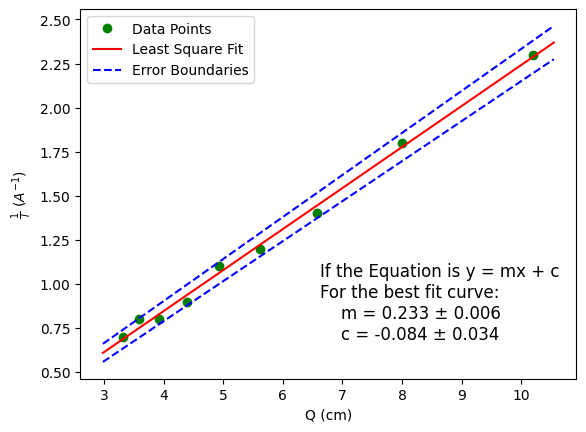
\includegraphics[width=0.45\textwidth]{graph1.png}
		\caption{Q vs. $\sfrac{1}{I}$ for $\nu = 13.42MHz$}
		\label{graph:1}
	\end{figure}

	\begin{figure}[H]
		\centering
		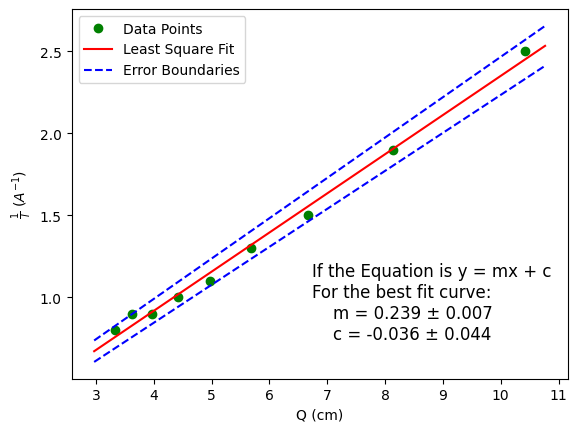
\includegraphics[width=0.45\textwidth]{graph2.png}
		\caption{Q vs. $\sfrac{1}{I}$ for $\nu = 14.34MHz$}
		\label{graph:2}
	\end{figure}

	\begin{figure}[H]
		\centering
		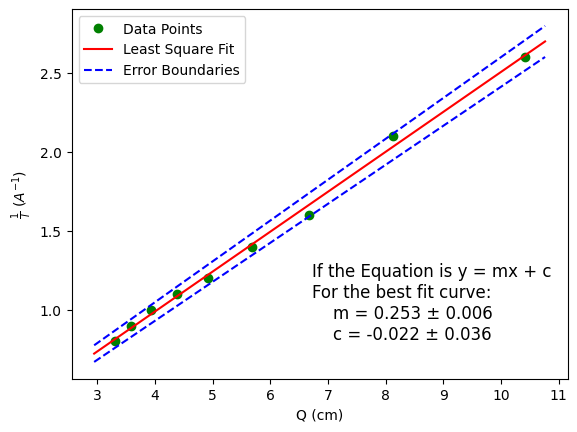
\includegraphics[width=0.45\textwidth]{graph3.png}
		\caption{Q vs. $\sfrac{1}{I}$ for $\nu = 15.44MHz$}
		\label{graph:3}
	\end{figure}

	
